% tickets.tex — генерация экзаменационных билетов по CSV

\foreach \num in {1,2,...,\DTLrowcount{questions}}
{

  \noindent
  \begin{center}
    \textbf{ \University }
  \end{center}
  \vspace{-0.5cm}
  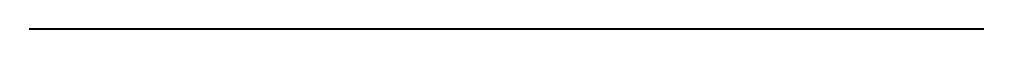
\begin{tikzpicture}
    \draw[thick] (0,0) -- (\textwidth,0);
  \end{tikzpicture}
  \begin{center}
    \textbf{ЭКЗАМЕНАЦИОННЫЙ БИЛЕТ № \num}\\
    \textbf{По дисциплине <<\Course>>}
  \end{center}

  \ifthenelse{\equal{\NumberOfQuestions}{2}}
  { % Если 2 вопроса в билете
    \begin{table}[h!]
      \centering
      \begin{tblr}
      {
        width = \linewidth,
        colspec = {Q[37]Q[693]Q[210]},
        column{1} = {c},
        column{3} = {c},
        row{1}   = {c, m, font=\bfseries},
        row{2-4} = {\RowHeight mm},
        hlines,
        vlines,
      }
        № & Вопрос / задача & Максимальная оценка в баллах \\
        1 & \DTLgetvalue{\Question}{questions}{\num}{1}\Question & \OneQuestionMark \\
        2 & \DTLgetvalue{\Question}{questions}{\num}{2}\Question & \TwoQuestionMark
      \end{tblr}
    \end{table}
  }
  { % Если 3 вопроса в билете
    \begin{table}[h!]
      \centering
      \begin{tblr}
      {
        width = \linewidth,
        colspec = {Q[37]Q[693]Q[210]},
        column{1} = {c},
        column{3} = {c},
        row{1}   = {c, m, font=\bfseries},
        row{2-4} = {\RowHeight mm},
        hlines,
        vlines,
      }
        № & Вопрос / задача & Максимальная оценка в баллах \\
        1 & \DTLgetvalue{\Question}{questions}{\num}{1}\Question & \OneQuestionMark \\
        2 & \DTLgetvalue{\Question}{questions}{\num}{2}\Question & \TwoQuestionMark \\
        3 & \DTLgetvalue{\Question}{questions}{\num}{3}\Question & \ThreeQuestionMark
      \end{tblr}
    \end{table}
  }

  \vspace{-0.5cm}
  \noindent
  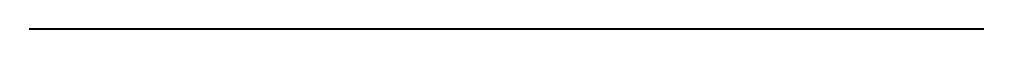
\begin{tikzpicture}
    \draw[thick] (0,0) -- (\textwidth,0);
  \end{tikzpicture}
  \noindent
  \footnotesize
  \textit
  {
    Билет рассмотрен и утвержден на заседании кафедры
    от \DecreeDate{}г. протокол № \DecreeNumber
  }

  \vspace{0.9cm}
  \noindent
  \textbf{Заведующий кафедрой \Department \hfill \HeadOfDepartment}

  \ifthenelse{\equal{\IsPrintCropLine}{true}}
  {
    \noindent
    \begin{center}
      \begin{tikzpicture}
        \draw[dashed] (0,0) -- (\textwidth,0);
      \end{tikzpicture}
    \end{center}
  }
  {}
  \pagebreak
}
